\documentclass{beamer}
\usepackage[T1]{fontenc}
\usepackage[utf8]{inputenc}
\usepackage[french]{babel}
\usepackage{lmodern}
\usepackage[squaren]{SIunits}
\usepackage{graphicx}
\usepackage{subfigure}
\newcommand{\Cbb}{\mathbb{C}}
\newcommand{\Nbb}{\mathbb{N}}
\newcommand{\Zbb}{\mathbb{Z}}
\newcommand{\Rbb}{\mathbb{R}}
\newcommand{\red}{\textcolor{red}}
\newcommand{\dr}{\partial}
\newcommand{\txt}{\text}
%\usepackage[font=scriptsize,labelfont=bf]{caption}
\usetheme{Warsaw}
\title[Project SF2520]{Project 8: Rotating Fluid in a cylinder}
\author{David \textsc{Weicker} \& Florentin \textsc{Goyens} }
\institute{KTH}
\date{18th December 2015}
\begin{document}

\begin{frame}
\titlepage
\end{frame}


\begin{frame}{Problem description}

\begin{itemize}
\item Rotating cylinder filled with water is stopped at $t=0$. Navier-Stokes equation in cylindrical coordinates 
\item Velocity only has angular component $\textbf{u}(r,\phi,z,t)=u_{\phi}(r,z,t)\textbf{e}_{phi}$
\item Symmetry of the domain $\rightarrow$ we consider a rectangular slice 
\end{itemize}

\begin{figure}[!h]
\centering
\includegraphics[width = 0.2\textwidth]{./cylindre.jpg}
\end{figure}

\end{frame}

\begin{frame}{Problem description}
Equation for $t>0$:
$$\dfrac{\dr u}{\dr t}= \nu\Big(\frac{1}{r}\frac{\dr}{\dr r}(r\frac{\dr u}{\dr r}) - \frac{u}{r^2} + \frac{\dr^2 u}{\dr z^2}\Big) \text{ for } 0<r<R \text{ and } 0<z<H.$$

Initial condition: 
$$u = \omega r \text{ for } 0\leq r \leq R$$

Boundary conditions: speed is zero on the boundary
$$u(r = 0) = u(r = R) = 0$$
$$u(z=0)= u(z=H) = 0$$
\end{frame}

\begin{frame}{High cylinder approximation}
\begin{itemize}
\item $u$ is assumed independent of $z$
\item Equation becomes:
\end{itemize}
$$\dfrac{\dr u}{\dr t}= f(u)= \nu\Big(\frac{1}{r}\frac{\dr u}{\dr r} + \frac{\dr^2 u}{\dr r^2} - \frac{u}{r^2}\Big)$$
\begin{itemize}
\item Parabolic equation %that requires implicit time-scheme\newline $\rightarrow$ \textsc{Crank-Nicholson}
\end{itemize}
\end{frame}

\begin{frame}{High cylinder approximation}
\begin{itemize}
\item Discretization of the domain with one spatial dimension
\end{itemize}
\begin{figure}[!h]
\centering
\includegraphics[width = 0.45\textwidth]{./MoL.jpg}
\end{figure}

\begin{itemize}
\item Discrete equation with 2nd order central finite difference
\end{itemize}
\begin{align*}
f(U_i ) &= \frac{\nu}{r_i}\dfrac{(U_{i+1}-U_{i-1})}{2h}+\nu\dfrac{U_{i+1}-2U_{i}+U_{i-1}}{h^{2}} -\frac{\nu}{r_{i}^2}U_{i}\\
&= \frac{\nu}{h}\Big( \frac{1}{h} - \frac{1}{2r_i}\Big)U_{i-1} 
 -\nu\Big( \frac{2}{h^2} + \frac{1}{r_{i}^{2}}\Big)U_{i}
+ \frac{\nu}{h}\Big( \frac{1}{h} + \frac{1}{2r_i}\Big)U_{i+1}\\
\end{align*} 
\end{frame}

\begin{frame}{High cylinder approximation}

\begin{itemize}
\item Tridiagonal matrix $f(U) = AU+b(t)$ with $b^t$ for boundary conditions
\item $b(t) =0$ for $t>0$ and $b(0)  = [0 \cdots 0  ~*]^{T}$ accounts for non zero initial condition at $r=R$.
\item ODE system $\dfrac{dU}{dt}=AU + b(t)$ is stiff ($h=R/10 \Longrightarrow \lambda_{max} = -0.0091, \lambda_{min}=-0.2571$), requires implicit method \textsc{Crank-Nicholson}
\end{itemize}
\end{frame}


\begin{frame}{High cylinder approximation}
\begin{itemize}
\item \textsc{Crank-Nicholson} method is of 2nd order
\end{itemize}
\begin{align*}
U^{t+1} &= U^{t} + 0.5*h_{t}\Big(f(U^{t}) + f(U^{t+1})\Big)\\
  &= U^{t} + 0.5*h_{t}\Big(A*U^{t}+b^t + A*U^{t+1} + b^{t+1}\Big)\\
\end{align*}
Therefore,
$$\Big(Id -0.5*h_{t}*A\big)U^{t+1} = (Id + 0.5*h_{t}*A)U^{t}+0.5*h_{t}*b^t$$
\begin{itemize}
\item Linear system that can easily be solved for $U^{t+1}$ with sparse solver in Matlab
\end{itemize}
\end{frame}

\begin{frame}{High cylinder approximation}
\begin{itemize}
\item Solution in Matlab
\end{itemize}
\begin{figure}[!h]
\centering
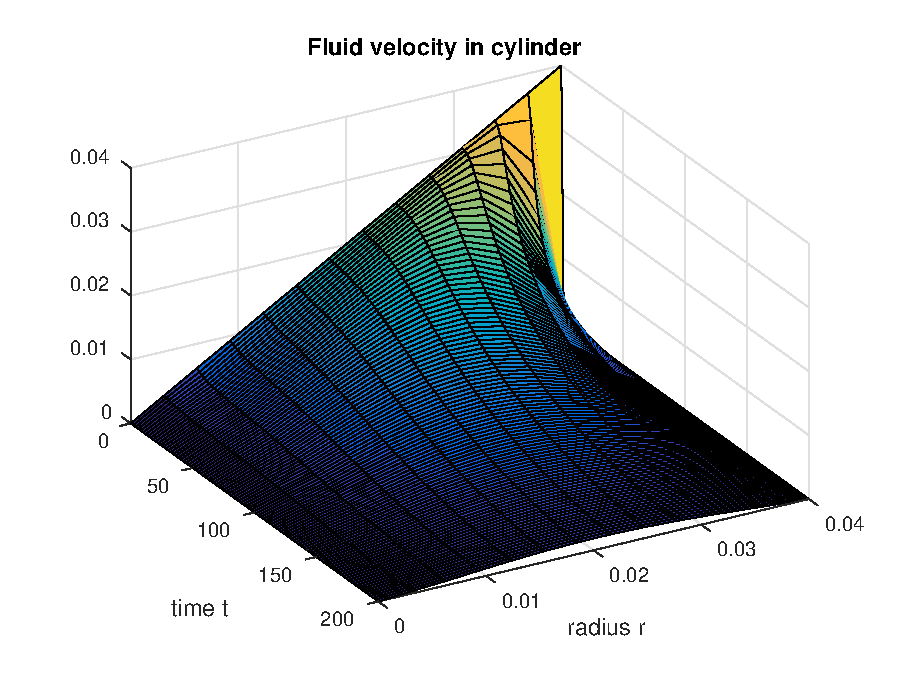
\includegraphics[width = 0.7\textwidth]{./dim1.eps}
\end{figure}
\end{frame}

\begin{frame}{High cylinder approximation: stability analysis}
Consider any perturbation of the form $U_{i}^{t}= U^{t}e^{jkr_i}.$
Define the constants $a_i=\frac{\nu}{h^2}\Big(1-\frac{1}{2i}\Big)$, $b_i=\frac{-\nu}{h^2}\Big(2+\frac{1}{i^2}\Big)$ and $c_i=\frac{\nu}{h^2}\Big(1+\frac{1}{2i}\Big)$. The scheme is 
$$\frac{U_{i}^{t+1}-U_{i}^{t}}{\Delta t}=\frac{1}{2}\Big( a_{i}U_{i-1}^{t}
+b_{i}U_{i}^{t}+c_{i}U_{i+1}^{t}
+ a_{i}U_{i-1}^{t+1}
+b_{i}U_{i}^{t+1}+c_{i}U_{i+1}^{t+1}\Big).$$
Plugging the ansatz gives
$$\Big(\frac{1}{\Delta t} -\frac{a_i}{2}e^{-jkh} -\frac{b_i}{2} -\frac{c_i}{2}e^{jkh}\Big)U^{t+1}=\Big(\frac{1}{\Delta t} +\frac{a_i}{2}e^{-jkh} +\frac{b_i}{2} +\frac{c_i}{2}e^{jkh}\Big)U^{t} .$$
 We get a stable scheme when the factor that amplifies perturbations has a complex module smaller than 1
 $$\dfrac{|U^{t+1}|}{|U^t|}\leq 1$$
\end{frame}
\begin{frame}{High cylinder approximation: stability analysis}

Let $\beta = \dfrac{a_ie^{-jkh} +b_i +c_ie^{jkh}}{2}$,
$$\dfrac{|1+\Delta t \beta|}{|1-\Delta t \beta|}\leq 1$$

$$\dfrac{Re\{1+\Delta t \beta\}^2 + Im\{1+\Delta t \beta\}^2 }{Re\{1-\Delta t \beta\}^2 + Im\{1-\Delta t \beta\}^2}\leq 1$$
Developments show that this will be satisfied when
$$a_i\cos(kh)+b_i + c_i \cos(kh)\leq 0.$$

This is indeed true because $a_i, c_i >0$ and
$$a_i\cos(kh)+b_i + c_i \cos(kh)\leq a_i + b_i + c_i = \frac{-\nu}{(ih)^2}< 0.$$

\end{frame}



\begin{frame}{2 dimensional problem}
\begin{itemize}
\item Solution $u$ now depends on $z$, this gives 2 dimensions for the space grid
\end{itemize}
\end{frame}

\begin{frame}{2 dimensional problem}
Straightforward generalization of 1D case for domain and equation

\begin{figure}[!h]
\centering
\includegraphics[width = 0.5\textwidth]{./grid.jpg}
\end{figure}
\begin{align*}
\dfrac{dU_{i,j}}{dt}&= \frac{\nu}{r_i}\dfrac{(U_{i+1,j}-U_{i-1,j})}{2h}+\nu\dfrac{U_{i+1,j}-2U_{i,j}+U_{i-1,j}}{h^2}\\ &\quad-\frac{\nu}{r_{i}^2}U_{i,j} 
+\dfrac{U_{i,j+1}-2U_{i,j}+U_{i,j-1}}{h^2} 
\end{align*}
\end{frame}

\begin{frame}{2 dimensional problem: solution}

\begin{figure}[!h]
\centering
\includegraphics[width = 1.1\textwidth]{./plot2D.eps}
\end{figure}

\end{frame}


\begin{frame}{Comparison of the 2 solutions}
\begin{itemize}
\item We want to discuss the decision to consider $z$-dependency
\end{itemize}

\begin{figure}[!h]
\centering
\includegraphics[width = 1.0\textwidth]{./compare.eps}
\end{figure}
\end{frame}

\begin{frame}
\begin{center}
Thank you for your attention
\end{center}
\end{frame}


\end{document}